\documentclass{article}


\usepackage[top = 1cm, right=2cm, left=2cm]{geometry}
\usepackage{graphicx}
\usepackage{xepersian}
\settextfont{B Nazanin}
\setlatintextfont{CMU Serif}



\title{گزارش تکلیف درس یادگیری ماشین}
\author{امیرحسین ابوالحسنی\\
400405003}
\date{
	پاییز 1403
	}
	
	
% Commands
\newcommand{\column}[1]{\lr{\textit{#1}}}


\begin{document}
	\maketitle
	
	\section*{مقدمه}
	تحلیل اکتشافی داده‌ها، یا
	\lr{Exploratory Data Analysis (EDA)}،
	به معنی بررسی داده‌ها به صورت آماری، پاکسازی داده ها و مصورسازی آنهاست، این کار یکی از مهمترین مراحل در یک پروژه می‌باشد.\\
	در این گزارش، به تحلیل دیتاست مشخصات مسافران کشتی تایتانیک میپردازیم.
	
	\section*{روش کار}
	\subsection*{بررسی معنایی دیتاست}
	دیتاست تایتانیک، متشکل از 11 ستون و 1309 نمونه می‌باشد.\\
	در اینجا معنی هریک از ستون‌ها ارائه می‌گردد:‌
	
	\begin{center}
		
			\begin{tabular}{c|c|c}
			نگاشت & توضیح & ویژگی\\
			\hline
			\hline
			0 : مرده ، 1 : زنده& نجات یافتن & \column{Survived}\\
			 1 : درجه یک ، 2 :‌ درجه دو ، 3 : درجه سه & نوع بلیط & \column{Pclass}\\
			 0 : زن ، 1 : مرد & جنسیت & \column{Sex}\\
			  & سن به سال،‌ برای کودکان زیر یک سال به صورت اعشاری می‌باشد. & \column{Age}\\
			  & تعداد همسر، خواهر و برادر سوار بر کشتی & \column{SibSp}\\
			  & نعداد والدین و فرزندان سوار بر کشتی & \column{ParCh}\\
			  & شماره بلیط & \column{Ticket}\\
			  & هزینه بلیط مسافر & \column{Fare}\\
			  & شماره کابین & \column{Cabin}\\
			  \lr{C = Cherbourg, Q = Queenstown, S = Southampton}
			  & بندر محل سوار شدن & \column{Embarked}\\
			\end{tabular}	
	\end{center}

	\subsection*{جمع آوری و تمیز کردن دیتا}
	با توجه به اینکه ستون تارگت از فایل 
	\lr{test.csv}
	جدا شده و در فایل 
	\lr{gender submission.csv}
	قرار دارد، ابتدا با عملگر پیوند داخلی این دو دیتافریم را با با یکدیگر جوین می‌کنیم، دیتا فرم به دست آمده با 
	\lr{train.csv}
	کانکت شده و همه داده‌ها در یک دیتاست قرار می‌گیرند.\\
	در مرحله بعد ویژگی‌های 
	\column{Cabin, Ticket, Name}
	را از دیتاست حذف می‌کنیم، با این استدلال که این سه ستون ربطی به نجات یافتن و یا مرگ مسافر به صورت مستقیم ندارد.\\
	
	\subsection{مقادیر هیچ‌مقدار}
	همانطور که در شکل 
	\ref{fig: nullHist}
	و
	\ref{fig: nullpies}
	دیده می‌شود، در دیتاست ستون‌های 
	\column{Age, Fare, Embarked, Cabin}
	دارای مقادیر هیچ‌مقدار می‌باشند.
	روش استفاده شده برای هر ستون به شرح زیر است:‌
	\begin{itemize}
		\item \column{Cabin}:
		این ستون در بخش قیل حذف شده است.
		
		\item \column{Fare}:‌
		از آنجایی که اثرگذارترین مشخصه ها در هزینه سفر، بدیهتا نوع بلیط و جنسیت می‌باشد و همچنین تعداد آن کم می‌باشد، داده ها را بر اساس این دو ویژگی گروه‌بندی کرده
		\footnote{
			معادل
			\lr{GroupBy}
			در
			\lr{SQL}
		}
		 و سپس میانگین هر گروه (که یکتا می‌باشد) را محاسبه می‌کنیم. حال با توجه به ترکیبی که ستون‌های 
		 \column{Pclass, Sex}
		 برای هر نمونه که دارای مقدار هیچ‌مقدار در ستون 
		 \column{Fare}
		 می‌باشد ایجاد می‌کند، میانگین مناسب خودش را در آن سلول میدهیم.
		 \begin{figure}[h]
		 	\centering
		 	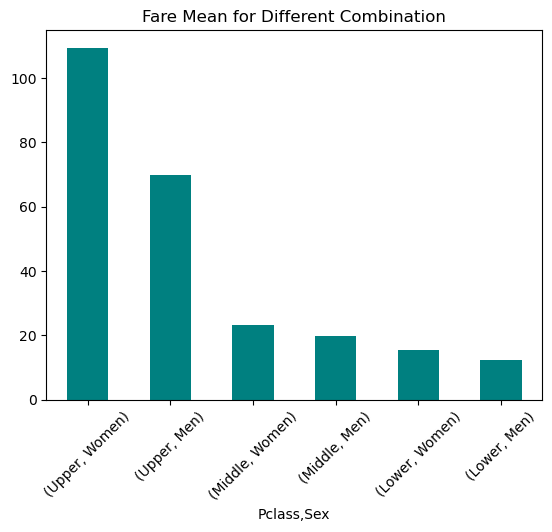
\includegraphics[scale=0.65]{./figs/Fare Mean for Different Combination}
		 	\caption{
		 		میانگین 
		 		\column{Fare}
		 		برای ترکیب‌های یکتای 
		 		\column{Pclass, Sex}
		 	}
		 	\label{fig:FareMean}
		 \end{figure}
		 
		 \item \column{Embarked}: 
		 برای پر کردن بعضی سلول‌های ستون 
		 \column{Embarked}،
		 دیتاست بر اساس ستون
		 \column{Pclass}		 
		 گروه‌بندی شده و فروانی هر بندر در هر یک از این گروه ها محاسبه می‌شود. سپس بر اساس مقدار ستون 
		 \column{Pclass}		 
		 برای هر نمونه دارای هیچ‌مقدار در این ستون، بندری گذشته می‌شود که بیشتر مسافران آن نوع بلیط از آنجا سوار بر کشتی شده اند.
		 
		 \item \column{Age}:
		 برای این ستون که بیشترین مقدار هیچ‌مقدار را در بین ستون‌های موجود دارد، از متد 
		 \lr{Iterative Imputation}
		 استفاده شده است. این متد سعی بر این دارد که این ویژگی را به عنوان تابعی از ویژگی های دیگر در دیتاست ببیند و با برقراری ارتباط بین آن‌ها(به کمک رگرسیون) سعی بر تخمین مقادیر سن با توجه به دیگر ویژگی‌های هر نمونه دارد.
	\end{itemize}
	
	
	
	\begin{figure}[!h]
		\centering
		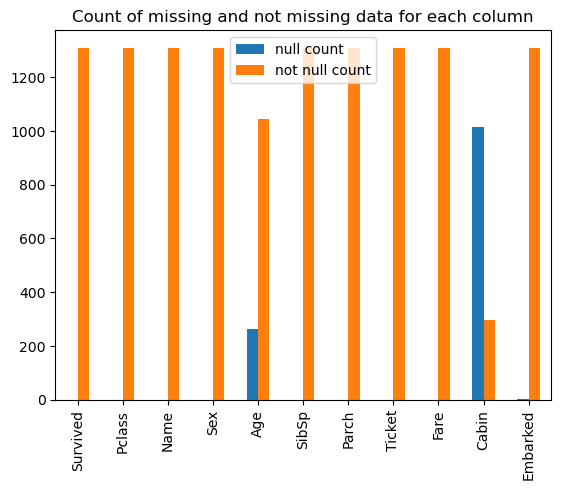
\includegraphics[scale=0.65]{./figs/Count-of-missing-and-not-missing data-for-each-column}
		\caption{
			فراوانی داده های هیج‌مقدار نسبت به داده‌های دارای مقدار برای هر ویژگی
		}
		\label{fig: nullHist}
	\end{figure}
	\begin{figure}[!h]
		\centering
		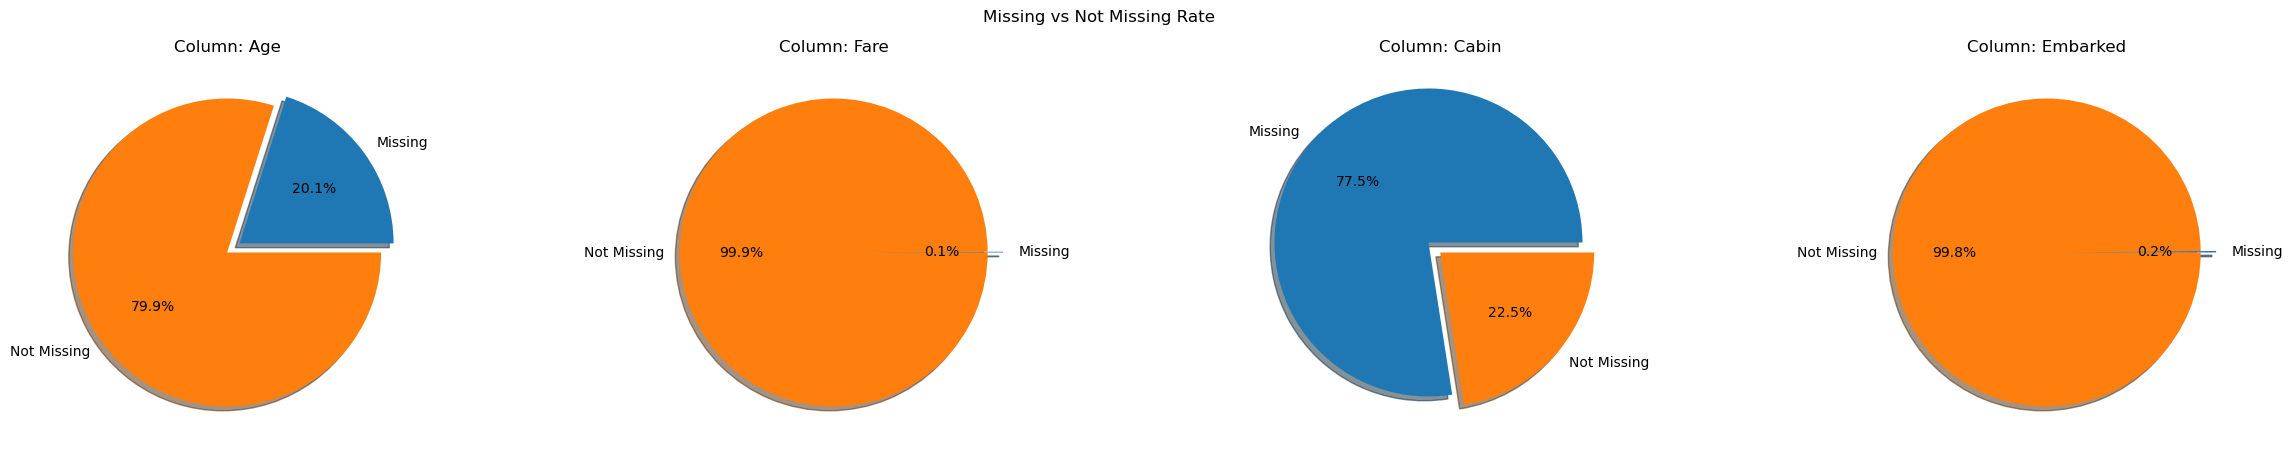
\includegraphics[scale=0.3]{./figs/Missing vs Not Missing Rate}
		\caption{
			نسبت داده‌های از دست داده شده به داده‌های موجود برای ستون‌های دارای مقادیر هیچ‌مقدار
		}
		\label{fig: nullpies}
	\end{figure}
	
	
	\section*{نتیجه گیری}
	لورم اپسیوم
	لورم اپسیوم
	\section*{منابع}
	لورم اپسیوم
	لورم اپسیوم
	
\end{document}